\begin{figure}[H]
  \centering
  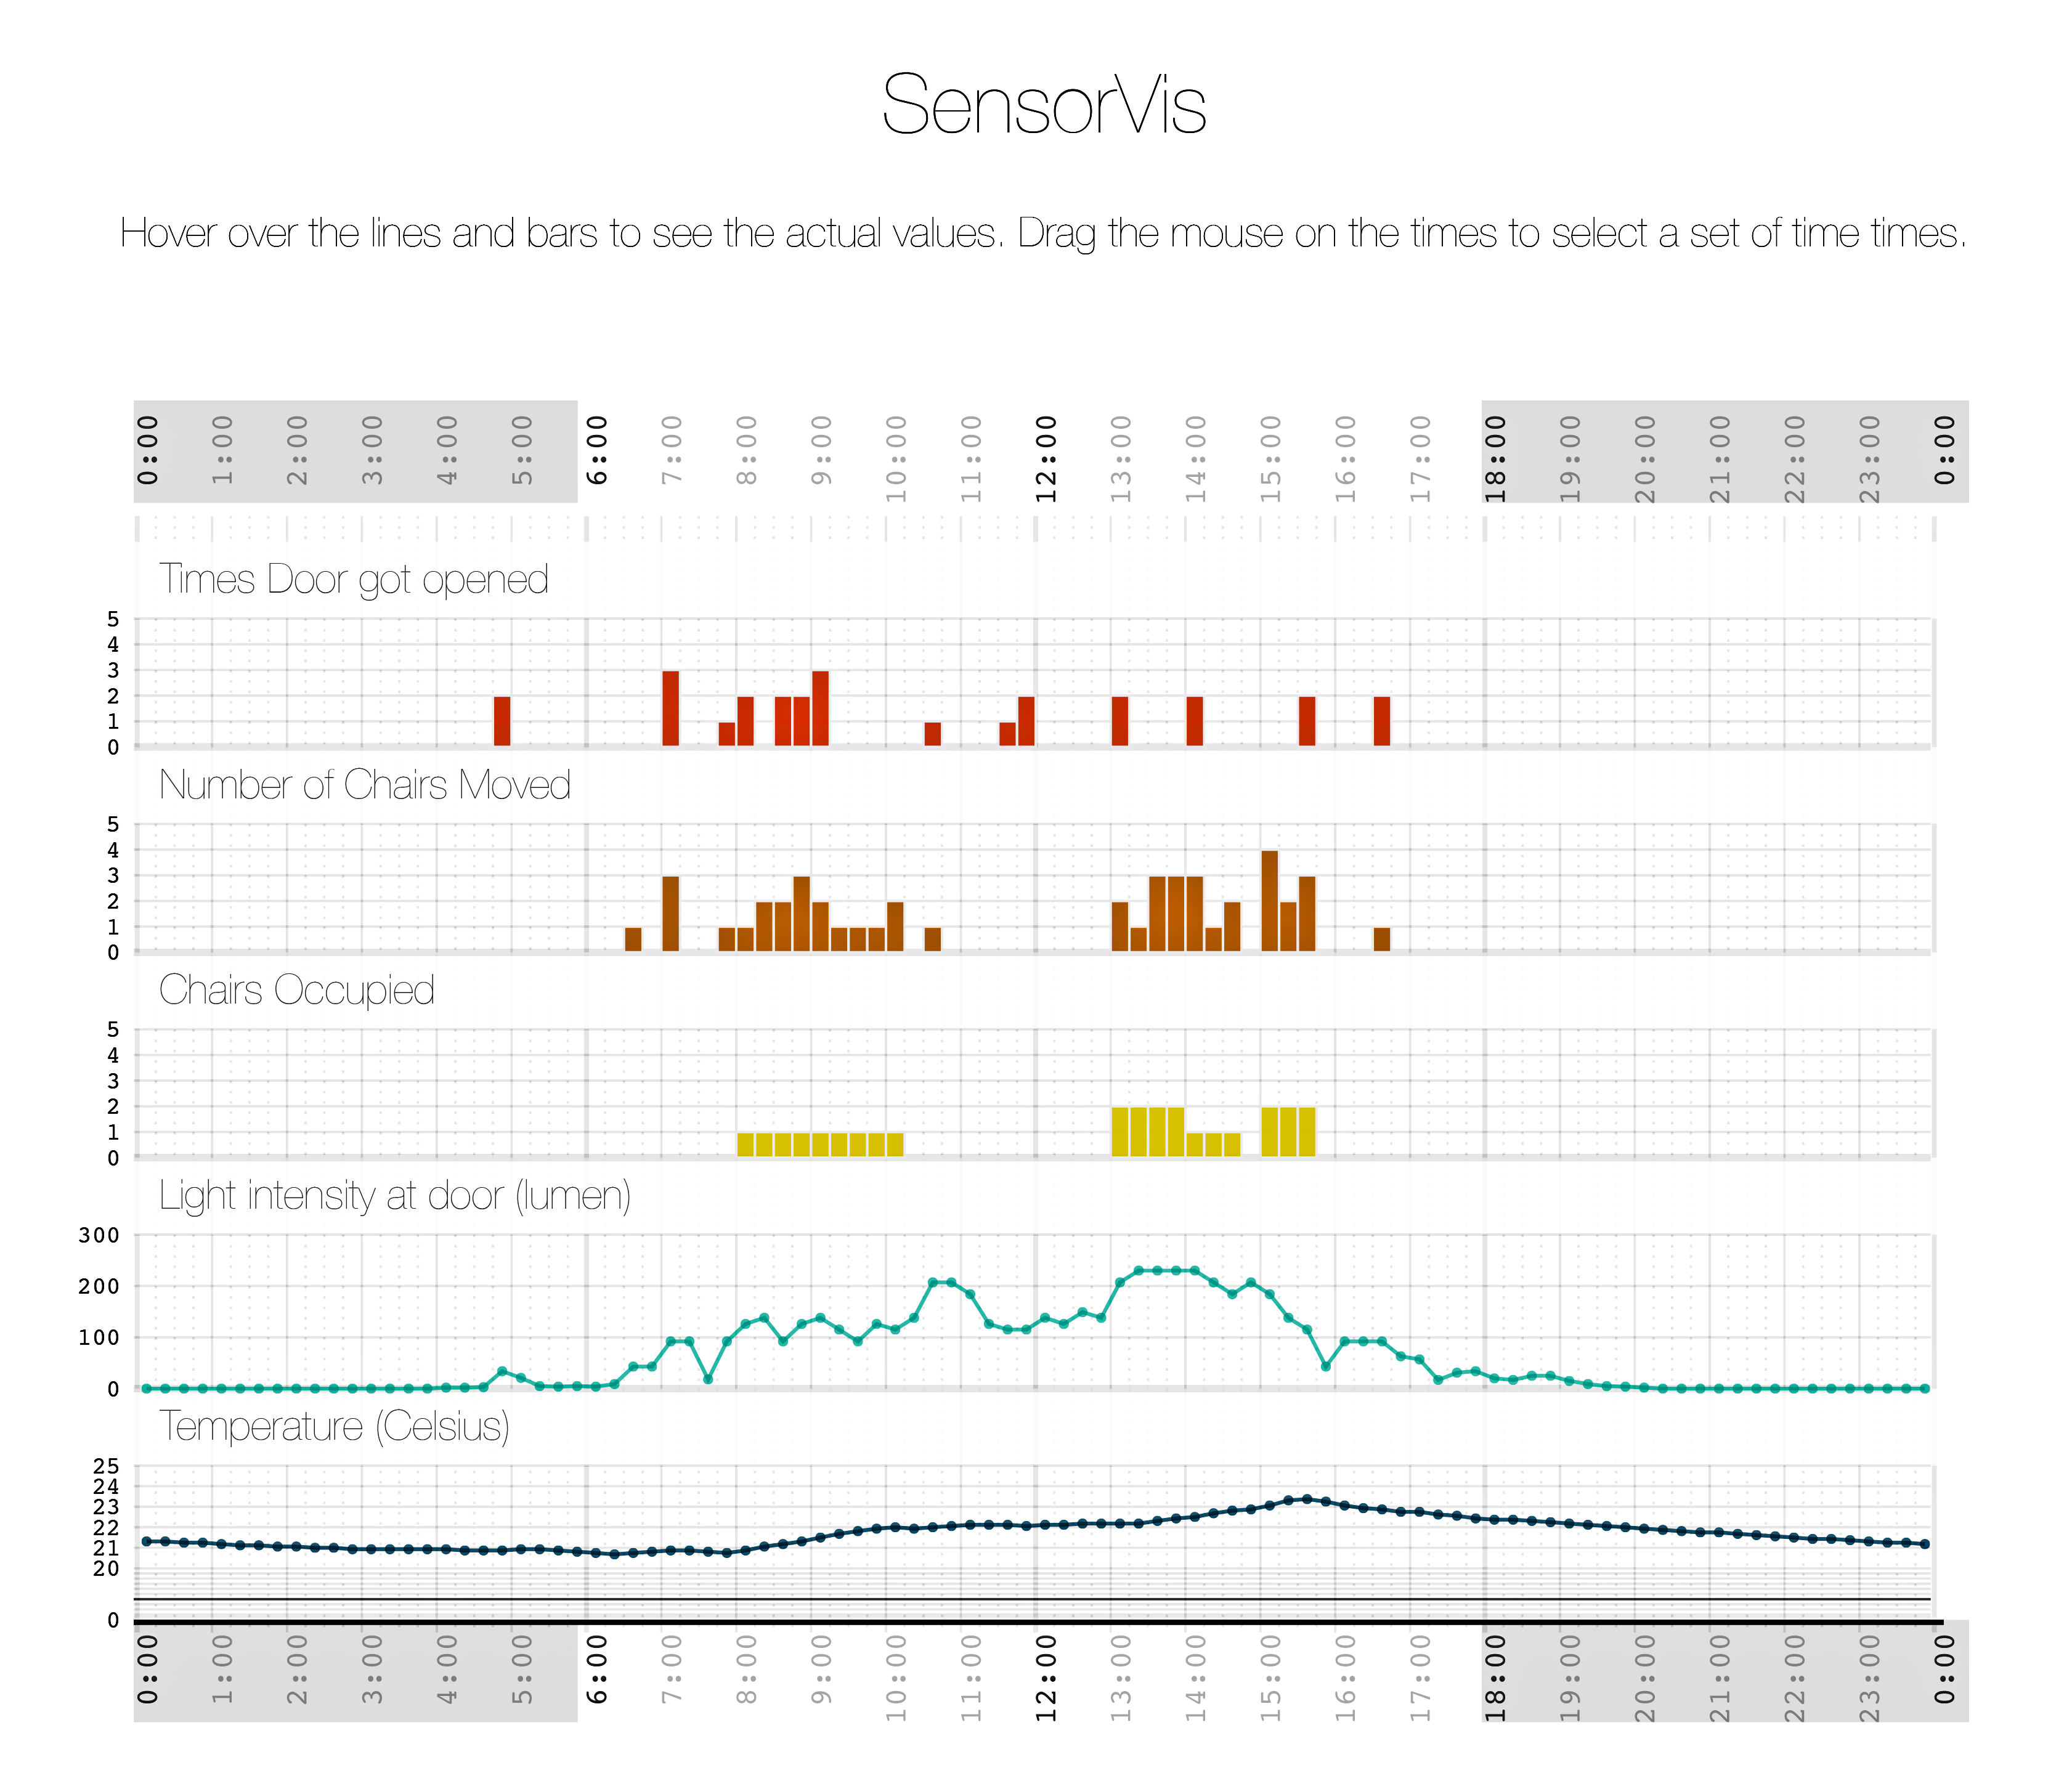
\includegraphics[scale=0.3]{images/occupancy.png}
  \caption{Screen dump of interactive data visualisation for a
    specific day. The $x$ axis shows the time dimension at 15 minute
    intervals over the course of the day. Horizontal bands show values
    for:  number of times the
    door was opened; the number of chairs that were moved; the number
    of chairs that were occupied; the light intensity in the room
    in lumens; and the temperature of the room in degrees Celsius.}
  \label{fig:dataviz}
\end{figure}

\subsection{Study Design}
\label{sec:study-design}

The main purpose of the study was to understand people’s qualitative
perceptions of monitoring in the workplace. We used semi-structured
interviews and focus groups to explore individual perspectives, organised around three main
questions:
\begin{enumerate}[noitemsep]
\item What do you know about the monitoring project and do you have
  any concerns about it?
\item What do you think are the main problems with the building and
  what would make your working environment better?
\item How do you view monitoring more broadly? What do you think about
  the use of data in various scenarios of building and office
  management?
\end{enumerate}


We adapted the interviews slightly from our
original plan to include a simple data visualisation, illustrating
a sample day’s data from the meeting room and demonstrating what categories of data were being
collected; cf.\ 
figure~\ref{fig:dataviz}.\footnote{
An online version of the visualization can be found at \url{http://www.aviz.fr/~bbach/occupancy/}.
}
We invited participants to reflect on the data visualisation and to
comment on what it revealed about human activities in the meeting
room. We also asked what they thought would be the impact of making
the monitoring data public through data visualisation: would it affect
staff perceptions of the monitoring and would it increase their
interest in engaging with the project?

\subsection{Participant Recruitment and Data Analysis}
\label{sec:recruitment}

Our candidate pool of study participants consisted of staff based in
the offices where the monitoring project was carried out. An email
from a senior manager was sent to all staff inviting them to
participate. A separate email was sent to managers in divisions to
highlight the study and ask them to encourage their staff to engage.
Due to low initial response, additional reminders were sent out.

We recruited nine interview participants and a total of six
participants for focus groups. One of the focus groups consisted of
two participants and the other of four, based on staff schedules and
availability. Some of the interviewees had heard of the monitoring
project and one had seen it come through a security review, but none
of them were directly involved with it.

Three interview participants were female and six
were male. Four focus group participants were female and two were
male. We did not ask people’s ages, but a general estimate is that
most participants were between 30 and 50 years of age.

We made audio recordings of the interviews, and used the
transcriptions and hand-written notes to analyse the data based on emerging themes.

%%% Local Variables: ***
%%% mode: latex ***
%%% coding: utf-8 ***
%%% TeX-engine: xetex ***
%%% TeX-master: "main.tex"  ***
%%% End: ***